\chapter{Result and Discussion} \label{result}

as we can see, the algorithm was able to finish a extreme scaled down version of the original sparse matrix. This is unfortunate, since our goal was to iterate over large graphs. But these results are still interesting and proves that HLS can be an improvement.
We were able to run a implementation with pipeline and loop unrolling, but that resulted in a too large core and the synthesiser took over 24 hour to synthesise, Which was too long and was therefore abandoned.
This resulted in that most of the numbers here are taken from Vivado HLS simulation and Cosimulation. |

\section{•}

\section{Performance}
As we can see, the hardware implementation is better then the C-simulated implementation, even at this low scale, we can see that the

We have here included a snapshot of our synthesis report. As we can see, we have a rather large utilization of look up table(LUT) and flip flop(FF). This is the result of the PIPELINE and Loop unrolling. Our high level implementation does contains several Loops and dependencies, this results in a large amount of resource used. 

We used the following variables to generate our adjacency matrix:
\begin{itemize}
\item \textbf{A} = 0.57
\item \textbf{B} = 0.19
\item \textbf{C} = 0.19
\item \textbf{D} = 1-0.57-0.19-0.19 = 0.05
\item \textbf{Edge factor}  = 16
\item \textbf{k (Scale)} = 4
\end{itemize}

By using the random-function provided by Python, we placed '1' in it's correct place. After the matrix is generated, we further applied a diagonal copying as shown in Figure:\ref{fig:flipDiagonal}. This is obligatory to generate an undirected graph.

For this project, a graph with size 1024 was used. This is a microscopic graph compared to graphs used in network analysis. 

\begin{figure}
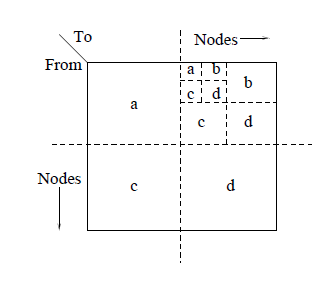
\includegraphics{Figures/Rmat}
\caption{The R-mat model \cite{Rmat2004}}
\label{fig:Rmat}
\end{figure}



\section{Discussion}
\subsection*{Analysis of the performance}
Our IP core was originally designed for networks with 1024 vertices, but after implementing with the optimization directives, the resource usage were out of bound. This resulted in a severe scale down for this project. The resulted network was down to the size of 16 vertices. In network analysis, this is such a small scale that the results from this experiment would only serve as a proof of concepts. 
 
\subsection*{problem that was encountered}
One problem that was encountered during this project was that the output signal from the synthesiser was not the correct direction. The output signal was often set as input signal. The HLS would automatically set the values as output signal or input signal.The reurn value from a funciton would be set as a the output signal, while the variable that the function takes, would be set as the input signal. Another way wo specify that something is the output signal would be to explicitly set them as pointer arguments. This will in set the signal to be output signal.

Another problem that I often encountered, was that the Vivado HLS often stop working. The problem was fixed by creating a new project and include the previous files.

Another problem, was that some times the Vivado HLS was not able to Cosimulate the implementation the first time. I was not able to find a solution to this problem except resynthesis the project. 

There were incidence where the implementation on the Zedboard did not behave as the implementation. This was solved by reprogramming the device and sometimes, restarting the Zedboard.

